\section{Wprowadzenie}

Rozdział zawiera podstawy teoretyczne związane z definicją i pomiarem zjawiska ubóstwa\footnote{Określenie ubóstwo w niniejszej pracy będzie używane wymiennie z określeniem niedostatek oraz bieda.}. Przedstawiono różne sposoby pojmowania ubóstwa, a także możliwe kryteria niedostatku. Następnie omówiono metody identyfikacji osób znajdujących się w sferze ubóstwa oraz wskaźniki umożliwiające pomiar tego zjawiska. Na podstawie źródeł literaturowych wyróżniono najistotniejsze determinanty biedy. W dalszej części rozdziału przedstawiono zjawisko ubóstwa w świetle realizowanych projektów administracyjnych oraz badawczych na poziomie międzynarodowym i krajowym. Pierwszy rozdział zamyka czasowa oraz przestrzenna analiza niedostatku w Polsce oparta na obecnie publikowanych źródłach danych.

\section{Definicja i sposób pomiaru}

Ubóstwo powszechnie identyfikowane jest z takimi zjawiskami jak bezrobocie, niepełnosprawność, bezdomność czy głód. Złożoność zjawiska ubóstwa przełożyła się na różnorodność w proponowanych w literaturze przedmiotu podejściach teoretycznych. W niniejszym rozdziale przedstawione zostaną te podejścia, które z punktu widzenia definicji ubóstwa i sposobu jego pomiaru odegrały w przeprowadzonych badaniach najistotniejszą rolę.

Rozbieżności z jakimi można się spotkać w ocenie zasięgu ubóstwa wynikają przede wszystkim z niejednoznaczności definicyjnych. Zjawisko ubóstwa jest szczególnie trudne do zdefiniowania ze względu na jego zmienność w czasie i przestrzeni. Gospodarstwo domowe, które obecnie znajduje się w sferze ubóstwa niekoniecznie musiało do niej przynależeć kilka lat wcześniej. Ponadto osoby ubogie mieszkające w krajach europejskich będą w dużo lepszej sytuacji materialnej aniżeli np. mieszkaniec Indii \citep{panek2011}.

W literaturze przedmiotu ubóstwo nieodłącznie związane jest z niezaspokojeniem pewnych potrzeb na oczekiwanym poziomie \citep{drewnowski1977}. Indyjski ekonomista i laureat Nagrody Banku Szwecji im. Alfreda Nobla, Amartya Sen wskazał, że ubóstwo to nie tylko niedostępność określonych dóbr i usług, ale także brak możliwości uczestnictwa w podejmowaniu decyzji oraz udziału w życiu społecznym i kulturalnym \citep{sen1992}. Kolejnym przykładem definicji ubóstwa może być ta zaproponowana przez Radę Wspólnoty Europejskiej, która stwierdza, że ``ubóstwo odnosi się do osób, rodzin lub grup osób, których zasoby (materialne, kulturowe i społeczne) są ograniczone w takim stopniu, że poziom ich życia obniża się poza akceptowalne minimum w kraju zamieszkania'' \citep{eec1985}.

\subsection{Sposób pojmowania ubóstwa}

Z punktu widzenia badań dotyczących zjawiska ubóstwa kluczowe jest określenie poziomu zaspokojenia potrzeb, który można uznać za oczekiwany. W tym kontekście ubóstwo można rozpatrywać w dwóch ujęciach --- absolutnym (bezwzględnym) lub relatywnym (względnym). Ubóstwo absolutne bazuje na określeniu konkretnych kategorii ilościowych i wartościowych jako stopnia zaspokojenia potrzeb. Dana jednostka (osoba, rodzina, gospodarstwo domowe) zostanie zaklasyfikowana jako uboga jeśli określone potrzeby nie będą na wystarczającym poziomie. W tym podejściu abstrahuje się od odniesienia poziomu zaspokojenia potrzeb danej jednostki do poziomu zaspokojenia potrzeb pozostałych członków populacji. Teoretycznie, ubóstwo absolutne może zostać wyeliminowane w momencie zaspokojenia potrzeb u wszystkich jednostek populacji. Może to nastąpić na drodze np. wzrostu ekonomicznego. Absolutne podejście do ubóstwa, mimo swojej nazwy, charakteryzuje się w pewnym stopniu relatywizmem. Zbiór podstawowych potrzeb oraz minimalny poziom ich zaspokojenia zależy bowiem m.in. od poziomu rozwoju społeczno-ekonomicznego analizowanego kraju.

Ubóstwo relatywne bazuje na odniesieniu poziomu zaspokojenia potrzeb jednostek do poziomu zaspokojenia tych potrzeb przez innych członków społeczeństwa. W tym przypadku ubóstwo jest związane z nadmiernymi różnicami w zaspokojeniu potrzeb przez jednostki w społeczeństwie. W~podejściu relatywnym ubóstwa nie można całkowicie wyeliminować. Ograniczenie tego zjawiska możliwe jest poprzez zmniejszaniu nierówności w zaspokajaniu potrzeb.

W praktyce podejście absolutne wykorzystywane jest w pracach Instytutu Pracy i Spraw Socjalnych (IPiSS) do określenia tzw. minimum egzystencji i minimum socjalnego. Z kolei podejście relatywne stosowane jest m.in. przez Główny Urząd Statystyczny (GUS).

Oba przedstawione podejścia mają pewne ograniczenia. Pojmowanie ubóstwa w sposób relatywny wiąże się brakiem stałego punktu odniesienia dla porównań zmian w czasie i przestrzeni. Z kolei w podejściu absolutnym problematyczne jest ustalenie zbioru podstawowych potrzeb oraz minimalnego stopnia ich zaspokojenia \citep{panek2013}.

\subsection{Kryteria ubóstwa}

Jednym z etapów w analizie ubóstwa jest ustalenie kryterium ubóstwa. W literaturze przedmiotu wyróżnia się dwa wiodące podejścia do tego zagadnienia: jednowymiarowe oraz wielowymiarowe. Stosując kryterium jednowymiarowe ocenia się stopień zaspokojenia potrzeb jednostki poprzez pryzmat dochodów (wydatków) wyrażonych w formie monetarnej. Zdefiniowane w ten sposób ubóstwo określane jest mianem ekonomicznego. Należy jednak zwrócić uwagę na niedoskonałość tego kryterium. W kategorii dochodu nie są ujęte przychody pozagotówkowe oraz majątek trwały. Ponadto deklarowany dochód jest często zaniżany poprzez zatajanie przychodów pochodzących z tzw. szarej strefy. Z kolei po stronie wydatków obserwuje się zaniżanie rozchodów na tytoń i~alkohol \citep{panek2004}.

Najważniejszym aspektem analizy ubóstwa jest określenie kryterium według, którego należy zaklasyfikować daną jednostkę (osobę lub gospodarstwo domowe) do sfery ubóstwa. W praktyce najczęściej stosowane jest kryterium dochodowe lub wydatkowe związane z ustaleniem granicy dochodów (wydatków) poniżej, których badana jednostka jest już uważana za ubogą. Wówczas analizowane zjawisko określane jest mianem ubóstwa ekonomicznego (monetarnego).

Ograniczenia podejścia jednowymiarowego oraz przekonanie, że ubóstwo jest w swej istocie zjawiskiem wielowymiarowym doprowadziły do tego, że wielu badaczy zaczęło postulować uwzględnienie w jego analizie także czynników pozamonetarnych. Wśród propozycji wymiarów ubóstwa, które miałyby zostać włączone do analizy znalazły się m.in. dochody i zasoby materialne nagromadzone w poprzednich okresach, warunki mieszkaniowe, edukacja oraz zasoby zawodowe i~finansowe \citep{panek2010}.

\subsection{Identyfikacja ubóstwa}\label{pr:identyfikacja-ubostwa}

W podejściu jednowymiarowym wyodrębnienie podpopulacji ubogich jednostek odbywa się z~wykorzystaniem pewnego krytycznego poziomu dochodów (wydatków) gospodarstw domowych określanego mianem granicy (linii) ubóstwa. Jednostka uznawana jest za ubogą, wówczas gdy poziom jej dochodów (wydatków) znajduje się poniżej przyjętej granicy ubóstwa.

Wyróżnia się następujące typy linii ubóstwa: granica absolutna, granica relatywna oraz granica subiektywna. Ponadto można także wyróżnić granicę ustawową, która zwykle jest wariantem jednej z wyżej wymienionych.

Granica absolutna jest wyznaczana jako wartość środków finansowych koniecznych do osiągnięcia minimalnego poziomu zaspokojenia potrzeb. Najczęściej w tej metodzie ustalany jest pewien koszyk towarów i usług, który umożliwia zaspokojenie potrzeb. W Polsce absolutnymi granicami ubóstwa są granica ubóstwa ustawowego, minimum socjalne oraz granica ubóstwa skrajnego (minimum egzystencji).

Ustawowa granica ubóstwa jest kwotą, która uprawnia do ubiegania się o przyznanie świadczenia z systemu pomocy społecznej. W ustawie z dnia 12 marca 2004 r. o pomocy społecznej (Dz. U. z 2008 r. Nr 115, poz. 728, z późn. zm.), w art. 8 ust. 1 ustalono, że prawo do świadczeń pieniężnych z~pomocy społecznej przysługuje osobie samotnie gospodarującej, której dochód nie przekracza 461 zł oraz osobie w rodzinie, w której dochód na osobę nie przekracza 316 zł. W~przypadku gdy dochód rodziny nie przekracza sumy kwot kryterium dochodowego na osobę w rodzinie, wówczas takiej rodzinie również przysługuje prawo do świadczeń. W artykule 9 niniejszej ustawy zaznaczono, że kryteria dochodowe będą weryfikowane co 3 lata przez Instytut Pracy i~Spraw Socjalnych.

Pierwsza weryfikacja odbyła się w roku 2006 i wówczas zwiększono kryterium dochodowe dla osoby samotnie gospodarującej do 477 zł (Rozporządzenie Rady Ministrów z dnia 24 lipca 2006 r. w sprawie zweryfikowanych kryteriów dochodowych oraz kwot świadczeń pieniężnych z~pomocy społecznej - Dz. U. Nr 135, poz. 950). Kolejna weryfikacja miała miejsce w roku 2009 (Dz. U. Nr 127, poz. 1055) i wówczas progi nie zostały zmienione. Rozporządzenie Rady Ministrów z~dnia 17 lipca 2012 r. (Dz. U. poz. 823) podwyższyło kryterium dochodowe dla osoby samotnie gospodarującej do wysokości 542 zł, a dla osoby w rodzinie do 456 zł. Następna zmiana miała miejsce w roku 2015 (Dz. U. poz. 1058), kiedy nastąpiła kolejna waloryzacja --- do poziomu 634 zł dla osoby samotnie gospodarującej oraz 514 zł dla osoby w rodzinie.

Oprócz konsultacji w zakresie wysokości granicy ubóstwa ustawowego, IPiSS wyznacza także koszyki minimum socjalnego oraz minimum egzystencji. Zgodnie z zamysłem autorów nie miały one stanowić linii ubóstwa, a jedynie wyznaczyć granicę wydatków gospodarstw domowych zapewniającą minimalnie godziwy poziom życia. Minimum socjalne jest kategorią potrzeb niezbędnych człowiekowi do odnawiania sił życiowych, posiadania i wychowania potomstwa oraz utrzymania więzi społecznych. Z kolei minimum egzystencji wyznacza granicę, poniżej której może nastąpić biologiczne zagrożenie życia. W wyznaczonym przez IPiSS koszyku dóbr i usług dla minimum socjalnego znalazły się następujące grupy potrzeb:

\begin{enumerate}
\item bytowo-konsumpcyjne (wyżywienie, mieszkanie, odzież, higiena i ochrona zdrowia, transport i łączność),
\item edukacyjne i kulturalne (wychowanie, edukacja, kultura),
\item rekreacyjno-wypoczynkowe (wypoczynek, sport, turystyka).
\end{enumerate}

Koszyk minimum egzystencji ogranicza się wyłącznie do potrzeb, które nie mogą zostać odłożone w czasie --- wyżywienie, mieszkanie, leki i higiena osobista, naprawa odzieży, edukacja dzieci w zakresie podstawowym. Dokładna charakterystyka obydwu koszyków znajduje się w pracy \citep{kurowski2002}.

Relatywna granica ubóstwa odnosi zamożność każdej jednostki do bogactwa pozostałych jednostek. Zwykle linię ubóstwa wyznacza się jako stałą część mediany lub średniej arytmetycznej dochodu (wydatków). Jednostka zostanie uznana za ubogą jeśli jej dochód będzie mniejszy od określonej, stałej części mediany lub średniej arytmetycznej rozkładu dochodów w całej populacji. Eurostat rekomenduje przyjęcie jako granicy ubóstwa 60\% mediany rozkładu dochodów \citep{eurostat2010}. Z kolei GUS w Badaniu Budżetów Gospodarstw Domowych wykorzystuje linię określoną jako 50\% średnich wydatków \citep{ubostwo-gus2013}. 

W podejściu subiektywnym jednostki same określają minimalny poziom konieczny do zaspokojenia potrzeb. 

\subsection{Wskaźniki ubóstwa}\label{pr:wskazniki-ubostwa}

Zapewnienie porównywalności dochodów pomiędzy gospodarstwami domowymi o różnym składzie demograficznym możliwe jest dzięki zastosowaniu skali ekwiwalentności. Wielkość ta określa o ile należy zmniejszyć lub zwiększyć dochód gospodarstwa o określonym składzie demograficznym, aby osiągnęło ono poziom konsumpcji odpowiedni dla gospodarstwa stanowiącego punkt odniesienia \citep{panek2007}.

W praktyce najczęściej stosowane są skale ekwiwalentności zaproponowane przez OECD \citep{atkinson2003}. Oryginalna skala OECD przyporządkowuje pierwszej osobie dorosłej wagę równą 1, każdej kolejnej osobie powyżej 14 roku życia wagę 0,7, natomiast osobom poniżej 14 lat wagę równą 0,5. Wartości skali można wyznaczyć z wykorzystaniem wzoru:

\begin{equation}
S_{70/50}=1+0,7(k_A-1)+0,5k_C,
\end{equation}

gdzie: $k_A$ - liczba osób powyżej 14 roku życia, $k_C$ - liczba osób poniżej 14 roku życia.

W połowie lat dziewięćdziesiątych wprowadzono zmodyfikowaną skalę OCED, która zaczęła być stosowana w krajach wysokorozwiniętych. Różni się ona od oryginalnej skali wagami przypisywanymi do kolejnych osób w gospodarstwie. W zmodyfikowanej skali OECD druga osoba dorosła ma przypisaną wagę 0,5, a osobom poniżej 14 roku życia przypisuje się wagę 0,3. Jest to związane z malejącym udziałem wydatków na żywność w budżetach gospodarstw domowych. Formalny zapis zmodyfikowanej skali OECD jest następujący:

\begin{equation}
S_{50/30}=1+0,5(k_A-1)+0,3k_C,
\end{equation}

gdzie: $k_A$ - liczba osób powyżej 14 roku życia, $k_C$ - liczba osób poniżej 14 roku życia.

Na podstawie wartości dochodów ekwiwalentnych można wyznaczyć odpowiednie miary ubóstwa. Ogólny wzór na wskaźniki ubóstwa został wyznaczony przez \citep{fgt1984} i od pierwszych liter nazwisk autorów tego artykułu przyjęło się określenie wskaźników FGT. W podejściu zakłada się, że dana jest skończona populacja $U={1,..., j, ..., N}$ podzielona na $D$ domen lub obszarów o liczebnościach $N_1, ..., N_D$. Wartość granicy ubóstwa określona jest przez $z$, natomiast $E_{dj}$ oznacza dochód $j$-tej jednostki w $d$-tej domenie. Jeśli $E_{dj} < z$, wówczas jednostka $j$ z obszaru $d$ określana jest jako znajdująca się w sferze ubóstwa. Ogólny wzór na wskaźniki ubóstwa z~rodziny FGT wyrażony jest następująco:

\begin{equation}
\label{eq:fgt}
F_{\alpha d}=\frac{1}{N}\sum\limits_{j=1}^{N_d}{\left(\frac{z-E_{dj}}{z}\right)^\alpha}I(E_{dj}<z), \alpha \geq 0, d=1, ..., D,
\end{equation}

gdzie: $I(E_{dj}<z) = 1$, jeśli $E_{dj}<z$ oraz $I(E_{dj}<z) = 0$ w przeciwnym przypadku.

Dla $\alpha=0$ otrzymuje się wskaźnik zasięgu ubóstwa określany również jako stopa ubóstwa. Z~kolei po podstawieniu $\alpha=1$ wynikiem jest głębokość ubóstwa (luka dochodowa), która informuje odległości dochodów osób ubogich od granicy ubóstwa. Innymi słowy, wskaźnik ten określa stopień ubóstwa osób ubogich.

W dalszej części rozdziału wskaźniki definiowane przez wzór (\ref{eq:fgt}) zostaną szczegółowo omówione.

\subsubsection{Stopa ubóstwa}

Odsetek osób ubogich w całej populacji jest najbardziej uniwersalną miarą ubóstwa i określany jest mianem zasięgu ubóstwa lub stopą ubóstwa. W raportach GUS można także spotkać się z~określeniem: wskaźnik zagrożenia ubóstwem. Podstawiając $\alpha=0$ w wyrażeniu (\ref{eq:fgt}) otrzymujemy 

\begin{equation}
\label{eq:hcr_linia}
F_0=\frac{1}{N}\sum\limits_{j=1}^{N}{I(E_{dj}<z)},
\end{equation}

gdzie: $F_0$ --- stopa ubóstwa, $N$ --- liczba osób w populacji, $E_{dj}$ --- dochód $j$-tej jednostki, $z$ --- granica ubóstwa, $I(.)$ --- funkcja indykatorowa przyjmująca wartość 1 jeśli wyrażenie wewnątrz funkcji jest prawdziwe i 0 w przeciwnym przypadku.

Alternatywnie stopę ubóstwa można zapisać jako:

\begin{equation}
\label{eq:hcr}
F_0=\frac{N_u}{N},
\end{equation}

gdzie: $F_0$ --- stopa ubóstwa, $N_u$ --- liczba osób poniżej granicy ubóstwa, $N$ - liczba osób w~populacji.

Wskaźnik zasięgu ubóstwa jest prosty w budowie i interpretacji --- informuje o odsetku osób ubogich w populacji. Niemniej jednak posiada przynajmniej trzy wady.

Po pierwsze stopa ubóstwa nie bierze pod uwagę intensywności ubóstwa. Analizując dwa wektory dochodów $A={100;100;150;150}$ i $B={124;124;150;150}$ oraz ustalając granicę ubóstwa na poziomie 125 okazuje się, że w obu przypadkach zasięg ubóstwa będzie taki sam - równy 50\%. Łatwo można jednak zauważyć, że większe ubóstwo występuję dla elementów wektora $A$.

Drugą wadą tego wskaźnika jest to, że jeśli osoby znajdujące się poniżej granicy niedostatku staną się jeszcze bardziej ubogie to stopa ubóstwa się nie zmieni. Przez to najprostszym sposobem redukcji stopy ubóstwa byłoby wsparcie z wykorzystaniem np. pomocy społecznej osób znajdujących się nieznacznie poniżej granicy ubóstwa. Biorąc pod uwagę standardy normatywne osoby będące nieco poniżej linii ubóstwa są tymi, które, z ekonomicznego punktu widzenia, najmniej cierpią z powodu niedostatku.

Trzecia niedoskonałość dotyczy ogólnego zalecenia mówiącego, że miary ubóstwa należy szacować dla osób, a nie gospodarstw. 20\% ubogich gospodarstw może w rzeczywistości oznaczać 25\% ubogiej populacji, jeśli ubogie gospodarstwa są liczne lub 15\% jeśli te gospodarstwa są małe.

Biorąc pod uwagę, że w większości badań reprezentacyjnych analizowane są gospodarstwa domowe przy przejściu na poziom osób należy przyjąć założenie, że wszystkie osoby w gospodarstwie charakteryzują się takim samym poziomem dobrobytu. Oczywiście w wielu sytuacjach nie będzie ono spełnione: starsi lub dzieci mogą być bardziej narażone na ubóstwo aniżeli pozostałe osoby w gospodarstwie \citep{haughton2009}.

\subsubsection{Głębokość ubóstwa}

Uzupełnieniem stopy ubóstwa jest głębokość ubóstwa (luka dochodowa), która informuje o poziomie ubóstwa wśród osób znajdujących się poniżej linii ubóstwa. Wzór na głębokość ubóstwa bazujący na formule (\ref{eq:fgt}) jest następujący:

\begin{equation}
\label{eq:pgi}
F_1=\frac{1}{N}\sum\limits_{j=1}^{N}{\left(\frac{z-y_i}{z}\right)I(E_{dj}<z)},
\end{equation}

gdzie: $F_1$ --- głębokość ubóstwa, $N$ --- liczba osób w populacji, $E_{dj}$ --- dochód $j$-tej osoby, $z$ --- granica ubóstwa, $I(.)$ --- funkcja indykatorowa przyjmująca wartość 1 jeśli wyrażenie wewnątrz funkcji jest prawdziwe i 0 w przeciwnym przypadku.

Wynik formuły \ref{eq:pgi} wyrażony jest jako procent granicy ubóstwa i interpretuje się go jako kwotę jaką przeciętnie należy dostarczyć ubogim, aby ich dochody przekroczyły linię ubóstwa. 

Na uwagę zasługuje również podejście, w którym głębokość ubóstwa oblicza się wyłącznie dla osób ubogich. Wówczas we wzorze (\ref{eq:pgi}) liczbę osób w populacji $N$ zastępuje się przez liczbę osób ubogich w populacji $N_u$. Tak obliczony wskaźnik informuje o przeciętnej zamożności osób ubogich. Tak zdefiniowaną głębokość ubóstwa publikuje Eurostat oraz GUS na podstawie danych z badania EU-SILC \citep{silc2017}.

\section{Determinanty ubóstwa}\label{pr:determinanty}

Niezbędnym elementem na drodze do redukcji poziomu ubóstwa jest identyfikacja jego symptomów. Haughton i Khandker [\citeyear{haughton2009}] wskazują na istnienie trzech poziomów, na których można obserwować kluczowe przyczyny ubóstwa:

\begin{itemize}
\item charakterystyki mierzone na poziomie regionalnym,
\item charakterystyki mierzone na poziomie środowiska lokalnego,
\item charakterystyki mierzone na poziomie jednostki (gospodarstwa domowego lub osoby), a~w~tym:
\begin{itemize}
\item demograficzne,
\item ekonomiczne,
\item społeczne.
\end{itemize}
\end{itemize}

Z kolei autorzy raportu \emph{Employment in Poland 2011 - Poverty and Jobs} \citep{mpra2013} dzielą przyczyny niedostatku na dwie grupy: lokalnej struktury gospodarczej oraz struktury demograficznej ludności lokalnej. W pierwszej grupie znajdują się m.in. stopa bezrobocia i przeciętne miesięczne wynagrodzenie brutto, natomiast w drugiej wskaźnik obciążenia demograficznego oraz oczekiwana długość życia w podziale na płeć.

Raport Instytutu Pracy i Spraw Socjalnych pt. \emph{Program przeciwdziałania ubóstwu i bezrobociu} \citep{kabaj2000} wskazuje na nadal aktualne przyczyny ubóstwa: długotrwałe bezrobocie, ograniczenie środków na programy rynku pracy, polaryzacja dochodów czy ograniczanie wydatków na pomoc społeczną.

Wyniki Diagnozy Społecznej \citep{diagnoza-panek2011} dowodzą, że największe ubóstwo obserwowane jest w grupach społeczno-ekonomicznych utrzymujących się z niezarobkowych źródeł (35,27\%) oraz tych, do których zaliczane są osoby bezrobotne (13,90\%). Wyższe wartości zasięgu ubóstwa obserwowane są także wśród rencistów (9,64\%) oraz rolników (8,98\%). Ze względu na typ gospodarstwa domowego najbardziej zagrożone ubóstwem są małżeństwa z co najmniej trojgiem dzieci (8,55\%) oraz rodziny niepełne (7,15\%). Jeśli uwzględni się wskaźnik głębokości ubóstwa to należy także wziąć pod uwagę gospodarstwa nierodzinne jednoosobowe (29,41\%) oraz małżeństwa z dwójką dzieci (27,12\%). Największym zasięgiem ubóstwa charakteryzują się także miasta poniżej 20 tys. mieszkańców (3,75\%) oraz wsie (6,44\%). Najlepsza sytuacja obserwowana jest w dużych miastach - powyżej 500 tys. mieszkańców (1,79\%).

Podobne wnioski dotyczące determinant ubóstwa można wysnuć na podstawie zastosowanego w badaniu Diagnoza Społeczna modelu probitowego. Oprócz wcześniej wymienionych uwzględniono w nim także cechy dotyczące wykształcenia oraz niepełnosprawności. Otrzymane wyniki wskazują, że nieposiadane wyższego wykształcenia zwiększa ryzyko znalezienia się w sferze niedostatku. Ponadto gospodarstwa z przynajmniej jedną osobą niepełnosprawną także charakteryzują się większym ryzykiem ubóstwa.

Główny Urząd Statystyczny w swoich publikacjach rozpatruje zjawisko ubóstwa w bardzo zbliżonych przekrojach społeczno-demograficzno-ekonomicznych. Przy czym GUS wśród typów gospodarstwa domowego rozpatruje także małżeństwa co najmniej czworgiem dzieci na utrzymaniu, dla których zasięg ubóstwa jest bardzo wysoki i w 2011 roku wynosił 47,5\% \citep{ubostwo-gus2013}. Uwzględnienie w ocenie stopy ubóstwa grup wiekowych pozwala zauważyć, że w grupie 0--17 lat obserwowane są wyższe wartości analizowanego wskaźnika (23,1\%) w porównaniu do osób wieku 18-64 lata (15,9\%) czy 65 lat i więcej (11,2\%). W pracy \textit{Jakość życia, kapitał społeczny, ubóstwo i wykluczenie społeczne w Polsce} \citep{jakosc-gus2013} opracowano model regresji logistycznej dla ubóstwa dochodowego. W kategorii głównego źródła utrzymania gospodarstwa domowego największe prawdopodobieństwo znalezienia się w sferze ubóstwa miały gospodarstwa utrzymujące się ze świadczeń społecznych oraz rent w odniesieniu do poziomu referencyjnego jakim była praca najemna. W omawianym opracowaniu uwzględniono w modelu także zawód głowy gospodarstwa domowego. Przyjmując za poziom referencyjny robotników przemysłowych oraz rzemieślników stwierdzono, że większe ryzyko ubóstwa dotyka osoby, które pracują jako rolnicy, ogrodnicy, leśnicy i rybacy, a także pracowników zatrudnionych przy pracach prostych. Najmniejsze prawdopodobieństwo ubóstwa odnotowano wśród kadry menedżerskiej, wyższych urzędników oraz kierowników.

% Ograniczanie ubóstwa jest jedną z funkcji świadczeń pieniężnych. Przyznawane są na podstawie kryterium dochodowego (pomoc społeczna) lub innych dodatkowych wymogów (zasiłek na dziecko). Wypłacane świadczenia mogą przyjmować różne formy, a ich celem jest wyrównywanie poziomu konsumpcji oraz wzmacnianie solidarności społecznej. Wypłacanie świadczeń jest związane ze sprawiedliwością społeczną i znajduje swoje odzwierciedlenie w konstytucji \citep{konstyt1997}. Wśród możliwych rozwiązań można wyróżnić następujące:

% \begin{itemize}
% \item świadczenia oparte na kryterium dochodowym,
% \item ulgi podatkowe dla osób pracujących,
% \item świadczenia rodzinne.
% \end{itemize}

\section{Problem ubóstwa we współczesnym świecie}\label{problem-ubostwa-we-wspoczesnym-swiecie}

Tematyka ubóstwa stanowi obszar zainteresowania wielu instytucji. Są to zarówno podmioty i~instytucje międzynarodowe, takie jak Unia Europejska czy Bank Światowy, organizacje działające na poziomie krajowym, lokalne samorządy oraz uniwersytety i inne jednostki badawcze.

\subsection{Projekty administracyjne}\label{projekty-administracyjne}

Podstawę  działań różnego rodzaju instytucji nakierowanych na walkę z ubóstwem stanowią ramy i uregulowania  prawne zawarte w projektach administracyjnych tych jednostek. I tak na przykład jako główny cel działania Banku Światowego oraz Organizacji Narodów Zjednoczonych zgodnie z Milenijnymi Celami Rozwoju jest eliminacja ubóstwa i głodu.

Traktat z Maastricht powołujący Unię Europejską w jednym z wyznaczonych celów wskazał walkę z ubóstwem przez Państwa Członkowskie w zakresie współpracy na rzecz rozwoju. Także Konstytucja Rzeczpospolitej Polskiej w artykule 71 wskazuje, że ''Rodziny znajdujące się w trudnej sytuacji materialnej i społecznej (\ldots{}) mają prawo do szczególnej pomocy ze strony władz publicznych'' \citep{konstyt1997}. W roku 2000 przyjęto plan rozwoju Unii Europejskiej określany mianem Strategii lizbońskiej. Głównym jego celem było utworzenie do roku 2010, na terenie Europy najbardziej konkurencyjnej gospodarki świata. Jednym z elementów tej strategii było także działanie w obszarze spójności społecznej. W 2010 roku dokonano rewizji postanowień Strategii lizbońskiej. Kryzys gospodarczy sprawił, że nie wszystkie cele udało się zrealizować w zadowalającym stopniu. Niemniej w ramach strategii utworzono 18 mln miejsc pracy, co wpłynęło na redukcję ubóstwa, ale jak wskazano w raporcie --- niektóre grupy społeczne mają nadal ograniczony dostęp do szkoleń dla nisko wykwalifikowanych osób.

Rok 2010 decyzją Unii Europejskiej został ogłoszony Rokiem Walki z Ubóstwem i Wykluczeniem Społecznym. Celem tej inicjatywy było podnoszenie świadomości obywateli Unii Europejskiej związanych ze zjawiskiem ubóstwa. W jej ramach zorganizowano szereg konferencji oraz kampanii informacyjnych. Na wszystkie działania podczas Roku Walki z Ubóstwem i Wykluczeniem Społecznym przeznaczono 17 mln euro.

Kontynuacją planu rozwoju z 2000 roku była ustanowiona dziesięć lat później Strategia Europa 2020 \citep{ke2010}. Impulsem do powołania tego programu był fakt, że po wielu latach wzrostu PKB Unii Europejskiej spadło o 4 punkty procentowe. Ponadto poziom produkcji wrócił do poziomu z lat dziewięćdziesiątych, a 10\% ludności w wieku produkcyjnym było bezrobotnych. Strategia Europa 2020 zakłada rozwój w trzech kluczowych obszarach:

\begin{itemize}
\item rozwój inteligentny,
\item rozwój zrównoważony,
\item rozwój sprzyjający włączeniu społecznemu.
\end{itemize}

W ramach każdego obszaru wyróżniono kilka skwantyfikowanych celów, które powinny zostać zrealizowane do roku 2020. Wśród nich znajduje się miedzy innymi osiągnięcie wskaźnika zatrudnienia na poziomie 75\% dla osób w wieku 20-64 lata, ograniczenie liczby osób przedwcześnie kończących naukę szkolną do poziomu 10\%, a także zapewnienie 40\% osobom z młodego pokolenia wyższego wykształcenia. W konkretnych ramach ilościowych zdefiniowano również zmniejszenie liczby osób zagrożonych ubóstwem --- o 20 mln osób.

Do realizacji ostatniego celu został powołany do życia projekt pt. ''Europejski program walki z ubóstwem''. Celem tego programu, stanowiącego kontynuację Europejskiego Roku Walki z~Ubóstwem i Wykluczeniem Społecznym, jest zapewnienie spójności gospodarczej, społecznej i~terytorialnej poprzez zwiększanie świadomości prawa do godnego życia i aktywnego uczestnictwa w~życiu społecznym wśród osób ubogich i wykluczonych społecznie.

Działania w ramach projektu odbywają się na dwóch poziomach: UE i państw członkowskich. Unia Europejska podejmuje się utworzenia instrumentu, który służyłby zachęcaniu podmiotów publicznych i prywatnych do działań mających na celu zmniejszenie wykluczenia społecznego, m.in. z wykorzystaniem funduszy strukturalnych, w tym Europejskiego Funduszu Społecznego. Innym zaproponowanym działaniem było opracowanie i wdrożenie programów wykorzystujących innowacje społeczne na rzecz osób w trudnej sytuacji społecznej. W gestii UE leżała także ocena adekwatności i trwałości systemów ochrony socjalnej oraz systemów emerytalnych, a także udoskonalenie dostępu do systemów opieki zdrowotnej.

Z kolei na barkach państw członkowskich znalazły się zadania, których celem było m.in. propagowanie poczucia odpowiedzialności za walkę z ubóstwem i wyłączeniem społecznym. Innym aspektem było wdrożenie działań rozwiązujących konkretne problemy grup szczególnie zagrożonych, takich jak samotni rodzice, osoby starsze czy niepełnosprawni i bezdomni. Na swoim poziomie państwa członkowskie miały także zapewnić wsparcie dochodu z wykorzystaniem systemów ochrony socjalnej i emerytalnej, a także dostępu do opieki zdrowotnej.

Weryfikacja realizacji celów strategii Europa 2020 w 2014 roku wykazała, że osiągnięcie zakładanego poziomu ubóstwa w 2020 roku może być trudne. Na rysunku \ref{fig:europa2020} przedstawiono stopę ubóstwa i wykluczenia społecznego w 27 krajach Unii Europejskiej oraz Polsce.

\begin{figure}[ht]
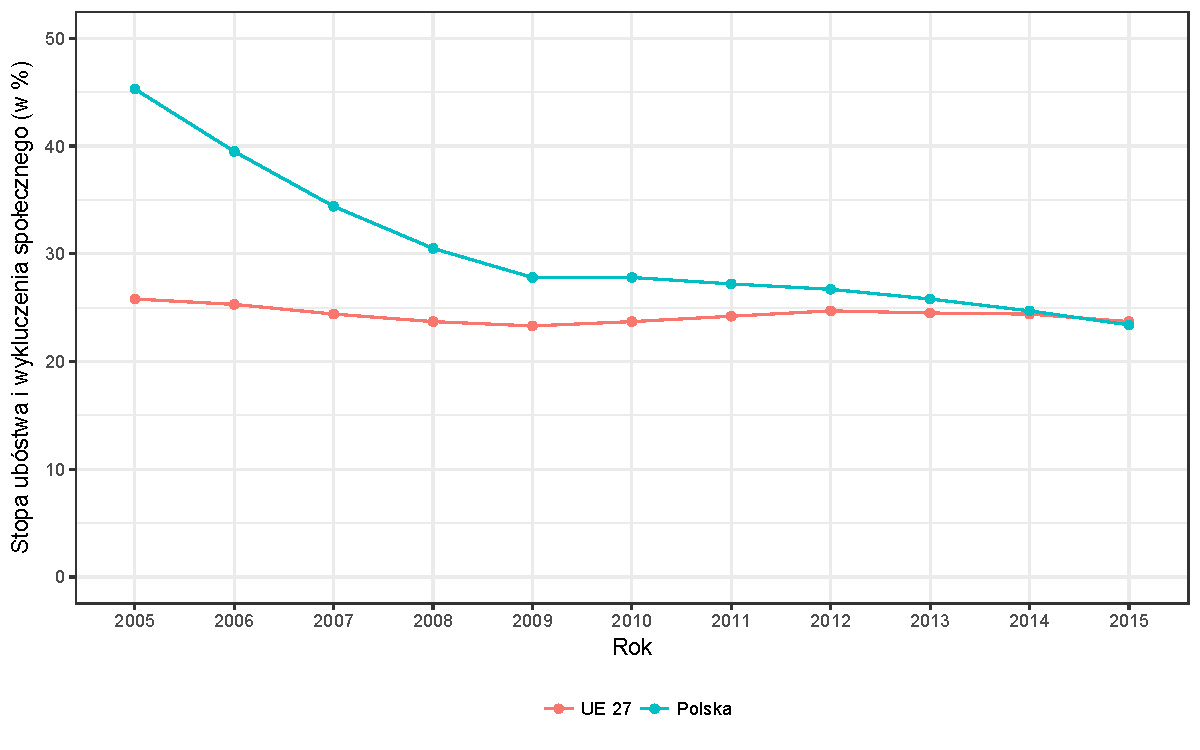
\includegraphics[width=\textwidth]{01_wykresy/europa2020-1.pdf}
\caption{Stopa ubóstwa i wykluczenia społecznego w latach 2005--2015 w Unii Europejskiej oraz Polsce}
\small{Źródło: opracowanie własne na podstawie danych Eurostatu.}
\label{fig:europa2020}
\end{figure}

W 2005 roku w Polsce prawie połowa populacji była zagrożona ubóstwem lub wykluczeniem społecznym. Od tego czasu wskaźnik ten systematycznie maleje i w roku 2015 kształtował się na poziomie nieznacznie niższym od wartości oszacowanej dla Unii Europejskiej. Niemniej oznacza to, że w Polsce żyje około 8,7 mln osób dotkniętych ubóstwem i wykluczeniem społecznym. Z kolei w UE wartość wskaźnika oscyluje w okolicy 25\% i utrzymuje się na stałym poziomie, co oznaczało około 117,6 mln osób żyjących w ubóstwie w 2015 roku. Biorąc pod uwagę fakt, że w 2010 roku w 27 krajach Unii Europejskiej żyło 116,82 mln ludzi ubogich, cel postawiony w Strategii Europa 2020 prawdopodobnie nie zostanie osiągnięty. O ile w Polsce ubóstwo maleje, trend wzrostowy odnotowywany jest w Estonii, Grecji, Hiszpanii, Portugalii, Słowenii czy Szwecji.

Narzędziem realizacji celów strategii Europa 2020 w Polsce jest Krajowy Program Reform powołany do życia w 2011 roku \citep{mr2011}. Zgodnie z tym dokumentem europejski cel strategii określony jako ``Zmniejszenie liczby osób zagrożonych ubóstwem lub wykluczeniem społecznym o 20 mln'' został dostosowany do polskiej sytuacji jako obniżenie o 1,5 mln liczby osób zagrożonych ubóstwem i/lub deprywacją materialną i/lub żyjących w gospodarstwach domowych bez osób pracujących lub o niskiej intensywności pracy. Działania w zakresie przeciwdziałaniu wykluczeniu społecznemu skupiają się przede wszystkim na zwiększaniu szans na zatrudnienie osób młodych, o niskim poziomie wykształcenia, złym stanie zdrowia, niepełnosprawnych czy imigrantów. Większość zadań została przekazana do realizacji Ministerstwu Pracy i Polityki Społecznej\footnote{Od 16 listopada 2015 roku Ministerstwo Rodziny, Pracy i Polityki Społecznej.}.

Raport z roku 2015 dotyczący postępów w zakresie przeciwdziałania ubóstwu zawiera informacje o zmniejszaniu się wskaźników ubóstwa i wykluczenia społecznego oraz przegląd podjętych działań. Wśród nich można wymienić m.in. nowelizację ustawy o promocji zatrudnienia i instytucjach rynku pracy, prowadzenie prac nad założeniami do ustawy o zmianie ustawy o pomocy społecznej czy wprowadzenie ustawy o Karcie Dużej Rodziny. Został także utworzony nowy program rozwoju pt. ``Krajowy Program Przeciwdziałaniu Ubóstwu i Wykluczeniu Społecznemu 2020. Nowy wymiar aktywnej integracji'' \citep{mr2015}.

Należy podkreślić, że działania prowadzone w ramach przedstaw wyżej przedsięwzięć nie koncentrują się przeciwdziałaniu ubóstwu poprzez świadczenia społeczne. Pomoc społeczna jest traktowana jako podstawowe narzędzie w ograniczaniu biedy, ale w rzeczywistości zwykle tylko zwiększa dochód obecny \citep{barr2016}. 

\subsection{Projekty badawcze}

Zjawisko ubóstwa jest także tematem badań wielu zespołów naukowców, których celem jest wypracowanie nowych metod analizy oraz nowych wskaźników mierzących niedostatek. W niniejszej części pracy zostaną zaprezentowane najważniejsze z nich.

\subsubsection*{SAIPE --- Small Area Income and Poverty Estimates}

Celem programu SAIPE jest dostarczenie oszacowań wskaźników ubóstwa dla szczegółowych przekrojów terytorialnych w Stanach Zjednoczonych. Docelowym poziomem estymacji są stany, hrabstwa oraz okręgi szkolne. Wykorzystując dane pochodzące z rejestrów administracyjnych, spisów powszechnych oraz badania reprezentacyjnego American Community Survey, amerykańskie biuro spisowe rokrocznie dostarcza rzetelnych oszacowań dla nieplanowanych domen. Wśród cech, które są szacowane znalazły się m.in. liczba osób dotkniętych ubóstwem, liczba dzieci życzących w ubóstwie w różnych grupach wieku oraz mediana dochodów gospodarstw domowych. Oszacowanie wartości tych zmiennych jest możliwe poprzez zastosowanie modelu Faya-Herriota oraz podejścia bayesowskiego. Metodologia programu jest nieustannie doskonalona w celu dostarczenia precyzyjnych szacunków ubóstwa. Na ich postawie lokalne władze zarządzają federalnymi programami pomocowymi \citep{saipe}.

\subsubsection*{AMELI --- Advanced Methodology for European Laeken Indicators}

Celem projektu realizowanego w latach 2008--2011 przez 10 instytucji europejskich był rozwój metodyki szacowania tzw. wskaźników lejkenowskich. Projekt składał się z 10 pakietów roboczych. Wykonawcy projektu w pierwszej kolejności określili aktualny stan wiedzy dotyczący wskaźników lejkenowskich. W przeglądzie literatury wskazują wykorzystanie analizowanych wskaźników w~różnych metodach, badaniach oraz publikacjach. Kolejny etap projektu dotyczył metod estymacji wskaźników za pomocą metod klasycznych oraz statystyki małych obszarów. W dalszej kolejności autorzy skupili się na metodach szacowania wariancji oraz estymacji odpornej. Kolejne pakiety robocze zawierały już wyniki przeprowadzonych obliczeń, których podstawę stanowiło badanie EU-SILC. Uzupełnienie raportów stanowi osiem pakietów napisanych w języku R \citep{ameli}

\subsubsection*{SAMPLE --- Small Area Methods for Poverty and Living Condition Estimates}

Podobnie jak projekt AMELI projekt SAMPLE był realizowany w latach 2008--2011 i także był finansowany w ramach siódmego programu ramowego w zakresie badań naukowych (7PR). W tej inicjatywie brały udział dwie polskie instytucje: Szkoła Główna Handlowa oraz Główny Urząd Statystyczny. Projektowi realizowanemu przez międzynarodowe konsorcjum przewodniczyła profesor Monica Pratesi (Uniwersytet w Pizie). W projekcie zaplanowano 6 pakietów roboczych. Celem pierwszego z nich był przegląd literatury dotyczącej wskaźników ubóstwa oraz weryfikacja podejść stosowanych w estymacji ubóstwa. Zaproponowano nowe podejście do estymacji ubóstwa bazujące na zbiorach rozmytych. Drugi pakiet roboczy zawierał opis istniejącej oraz nowej metodyki w zakresie estymacji ubóstwa dla nieplanowanych domen. Wszystkie metody zostały oprogramowane w języku R. Wypracowaną metodykę poparto przykładami na rzeczywistych danych pochodzących z badań EU-SILC przeprowadzonych we Włoszech oraz Hiszpanii. Następnie zespół projektowy zbadał dostępność danych dotyczących warunków życia oraz polityki społecznej na poziomie lokalnym. Celem czwartego pakietu roboczego było utworzenie oprogramowania umożliwiającego niewykwalifikowanym użytkownikom korzystanie z wypracowanych metod oraz wyników. Dwa ostatnie pakiety robocze dotyczyły spraw organizacyjnych \citep{sample}. 

\vspace{1em}

\noindent W Polsce także zrealizowano kilka projektów, których celem była estymacja wskaźników ubóstwa dla małych domen.

\subsubsection*{Wykluczenie i integracja społeczna w Polsce}

W projekcie prowadzonym we współpracy polskich naukowców z ośrodkami w Niemczech, Słowacji oraz Włoszech dokonano analizy wskaźnikowej wykluczenia społecznego. Jednym z elementów tej analizy było wykorzystanie metod statystyki małych obszarów do estymacji wybranych wskaźników na poziomie powiatów. W tym celu wykorzystano klasyczny model Faya-Herriota \citep{fh1979} oraz dane jednostkowe pochodzące z Badania Budżetów Gospodarstw Domowych. Szacowano dochód ekwiwalentny oraz dochód \textit{per capita}, a także logarytmy tych cech. Ponadto obliczono kompozytowy wskaźnik ubóstwa będący średnią ważoną wartości stóp ubóstwa dla granic określonych na poziomie 50\%, 60\% oraz 70\% mediany dochodów. W zastosowanych modelach znalazły się takie zmienne niezależne jak: odsetek osób z wykształceniem wyższym wśród osób w wieku 15--64 lata, odsetek bezrobotnych długookresowo (powyżej 1 roku) wśród bezrobotnych w wieku 15--64 lata, przeciętna liczba osób na 1 pokój (logarytm naturalny), odsetek ludności w~mieszkaniach zamieszkanych stale bez wodociągu czy odsetek osób w rodzinach z co najmniej 3~dzieci w wieku do lat 24 pozostających na utrzymaniu \citep{wykluczenie2006}.

\subsubsection*{Mapy ubóstwa na poziomie podregionów w Polsce z wykorzystaniem estymacji pośredniej}

Projekt realizowany w latach 2013--2014 przy udziale Banku Światowego, Głównego Urzędu Statystycznego oraz Urzędu Statystycznego w Poznaniu miał na celu oszacowanie wartości stopy ubóstwa w przekroju podregionów w Polsce. Na podstawie danych jednostkowych z badania EU-SILC 2011 oszacowano stopę ubóstwa z wykorzystaniem estymatora bezpośredniego. Wartości te stanowiły zmienną zależną w zastosowanym później modelu Faya-Herriota. Jako zmienne pomocnicze wykorzystano wskaźniki pochodzące z Narodowego Spisu Powszechnego Ludności i~Mieszkań 2011 oraz Banku Danych Lokalnych. W modelu znalazły się takie zmienne jak odsetek liczby osób samotnych powyżej 25 roku życia, liczba pokoi przypadająca na członka gospodarstwa domowego, odsetek gospodarstw domowych posiadających łazienkę, odsetek gospodarstw domowych z~dwiema osobami powyżej 25 roku życia z wykształceniem co najwyżej zawodowym, gęstość zaludnienia oraz stosunek liczby osób wymeldowanych do liczby zameldowanych na pobyt stały w~podregionie. W rezultacie uzyskano oszacowania pośrednie stopy ubóstwa na poziomie podregionów, charakteryzujące się lepszą precyzją aniżeli oszacowania otrzymane na podstawie estymatora bezpośredniego. Otrzymane wyniki wskazały na występowanie terytorialnego zróżnicowania ubóstwa --- wschodnia część kraju cechuje się wyższym odsetkiem osób ubogich w~porównaniu do części centralnej i zachodniej \citep{mapowanie2014}.

\subsubsection*{Pomiar ubóstwa na poziomie powiatów}

Praca badawcza była realizowana w latach 2013--2015 w ramach projektu o nazwie \textit{Statystyka dla polityki spójności} finansowanego ze środków Europejskiego Funduszu Rozwoju Regionalnego w ramach Programu Operacyjnego Pomoc Techniczna 2007--2013  --- oś priorytetowa 3  „Wsparcie realizacji operacji funduszy strukturalnych”, działanie 3.1 „Wsparcie instytucji zaangażowanych w realizację NSRO”. Celem projektu było oszacowanie stopy ubóstwa na poziomie powiatów w~latach 2005, 2008 oraz 2011. Projekt był podzielony na dwie części. W pierwszej, mającej charakter teoretyczny, zespół badawczy dokonał przeglądu literatury, wskazał możliwe źródła danych w~estymacji poziomu ubóstwa, przeprowadzono także kwerendę dotyczącą najistotniejszych zmiennych pomocniczych w estymacji stopy ubóstwa. W raporcie zawarto przegląd najważniejszych metod z zakresu statystyki małych obszarów oraz zaproponowano kilka narzędzi informatycznych użytecznych w estymacji ubóstwa. W drugim etapie przedstawiono teoretyczne aspekty pomiaru ubóstwa oraz uzupełniono opis zastosowanych estymatorów. Estymację stopy ubóstwa poprzedzono analizą taksonomiczną. Oszacowania stopy ubóstwa dla lat 2005, 2008 oraz 2011 na poziomie powiatów uzyskano wykorzystując jednostkowe dane z badania EU-SILC oraz wskaźniki z Banku Danych Lokalnych. Zastosowano estymatory uwzględniające korelacje w czasie oraz przestrzeni \citep{raoyu1994,faydiallo2012}. Ponadto dla roku 2011, z racji dostępności danych z Narodowego Spisu Powszechnego Ludności i Mieszkań 2011 oszacowano wartości stopy ubóstwa z wykorzystaniem estymatora EB \citep{ebp2010}. Na podstawie przeprowadzonych prac zespół badawczy zarekomendował dalsze rozwijanie metodologii szacowania ubóstwa na niskich poziomach agregacji przestrzennej w Polsce \citep{pomiar2015}.

\section{Ubóstwo w Polsce}

Ta część rozdziału poświęcona jest zjawisku ubóstwa wyłącznie w odniesieniu do Polski. W pierwszej kolejności przeanalizowano obowiązujące w naszym kraju kryteria ubóstwa w ujęciu czasowym. Na ich postawie obliczono wskaźnik zasięgu ubóstwa. W dalszej części omówiono przestrzenny wymiar ubóstwa w Polsce z uwzględnieniem podziału NUTS 2. Wizualizacje wartości stopy ubóstwa zaprezentowano w postaci kartogramów.

\subsection{Czasowy wymiar ubóstwa}\label{pr:czasowy-wymiar-ubostwa}

W Polsce można wyróżnić pięć kryteriów oceny ubóstwa: minimum socjalne, minimum egzystencji, ustawową granicę ubóstwa oraz relatywną granicę ubóstwa obliczaną na podstawie dwóch badań reprezentacyjnych (BBGD i EU-SILC). W tej części pracy przedstawiono porównanie wartości tych kryteriów oraz otrzymanych na ich podstawie wartości zasięgu ubóstwa wykorzystując dostępne dane z lat 2005--2015. Na rysunku \ref{fig:gr_1os} przedstawiono wyznaczone granice ubóstwa dla gospodarstwa jednoosobowego.

\begin{figure}[ht]
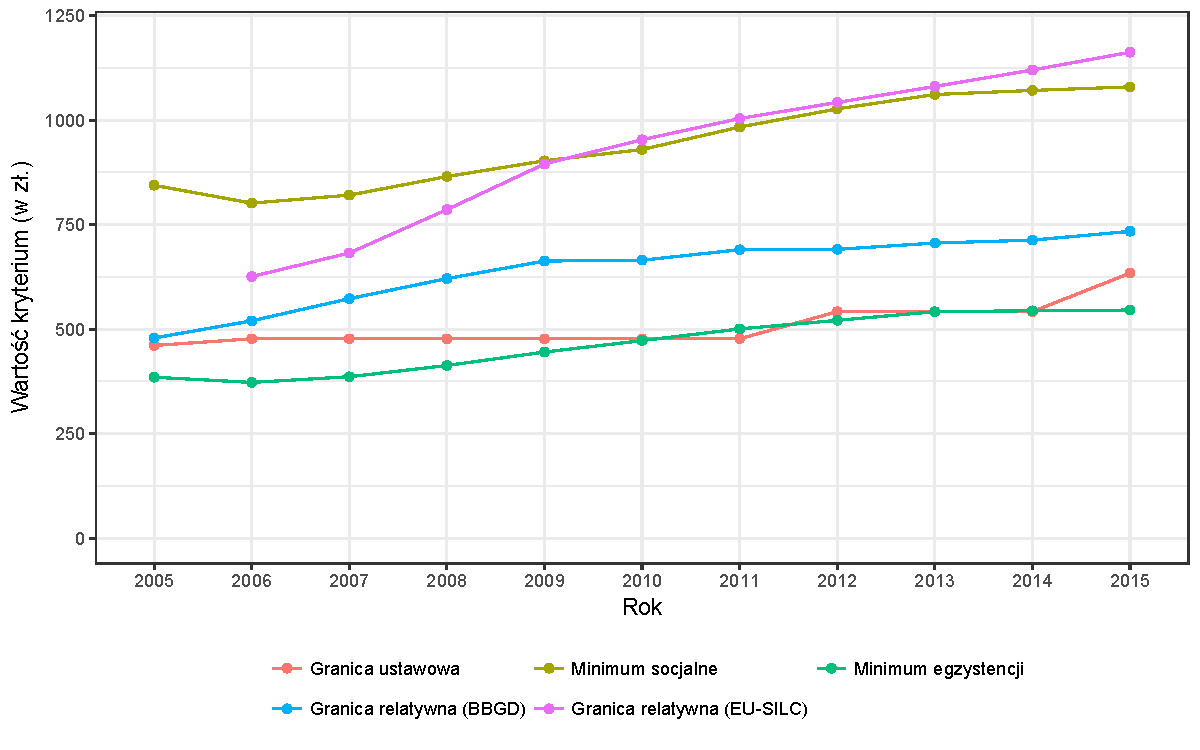
\includegraphics[width=\textwidth]{01_wykresy/gr_1os-1.pdf}
\caption{Granice ubóstwa dla gospodarstwa jednoosobowego w latach 2005--2015 w Polsce}
\small{Źródło: opracowanie własne na podstawie danych GUS, IPiSS oraz MRPiPS.}
\label{fig:gr_1os}
\end{figure}

Analizując wartości przedstawione na rysunku \ref{fig:gr_1os} należy zwrócić uwagę na kilka aspektów. Granica ubóstwa ustawowego oraz relatywnego obliczona na podstawie EU-SILC w odróżnieniu od pozostałych wartości opiera się na dochodach, a nie wydatkach. Ponadto wartości dla tej drugiej granicy dostępne są dopiero od roku 2006, ponieważ dopiero od tego roku wtedy GUS zaczął realizować badanie EU-SILC. Interpretacja wartości przestawionych na rysunku pozwala na zaobserwowanie pewnych zależności. Widoczne jest podobieństwo pomiędzy poziomem granicy ubóstwa ustawowego oraz ubóstwa skrajnego. Podobnie w przypadku wartości minimum socjalnego oraz relatywnej granicy ubóstwa dla EU-SILC --- od roku 2009 obie wartości kształtują się na podobnym poziomie. Natomiast granica ubóstwa relatywnego wyznaczona jako 50\% średniej wydatków jest wyższa od minimum egzystencji i granicy ubóstwa ustawowego, ale niższa od minimum socjalnego i granicy ubóstwa relatywnego wyznaczonego jako 60\% mediany dochodu.

Rysunek \ref{fig:gr_4os} przedstawia granice ubóstwa dla gospodarstwa 4-osobowego.

\begin{figure}[ht]
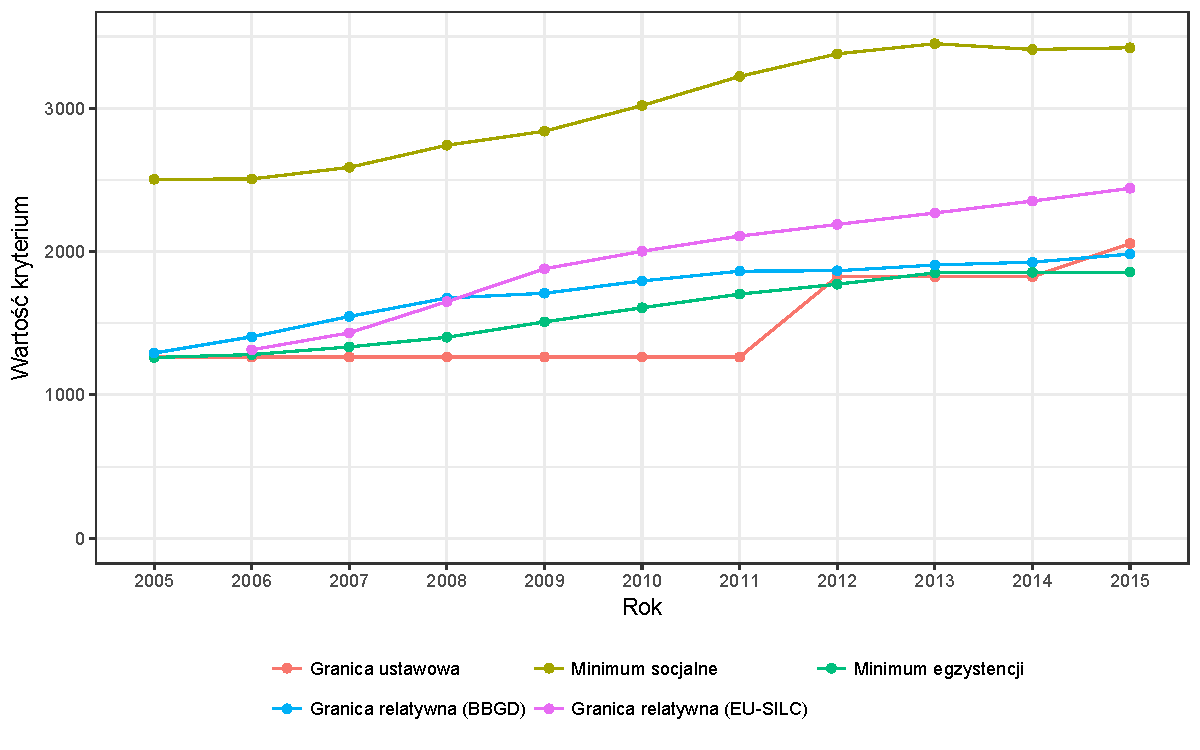
\includegraphics[width=\textwidth]{01_wykresy/gr_4os-1.pdf}
\caption{Granice ubóstwa dla gospodarstwa 4-osobowego w latach 2005--2015 w Polsce}
\small{Źródło: opracowanie własne na podstawie danych GUS, IPiSS oraz MRPiPS.}
\label{fig:gr_4os}
\end{figure}

W tym przypadku widoczny jest podział analizowanych granic ubóstwa na dwie grupy o~podobnych wartościach. Najniższymi wartościami cechują się granice ubóstwa ustawowego oraz skrajnego, które w poszczególnych latach się przecinają. Wyższymi wartościami od granic już wymienionych cechują granice ubóstwa relatywnego wyznaczone na podstawie BBGD i EU-SILC. Mimo znaczących różnic metodycznych obie z nich kształtują się na podobnym poziomie. Wyraźnie wyższa jest z kolei wartość minimum socjalnego.

Na rysunku \ref{fig:gr_stopa_ub} przedstawiono wartości stopy ubóstwa biorąc pod uwagę wcześniej scharakteryzowane granice ubóstwa.

\begin{figure}[ht]
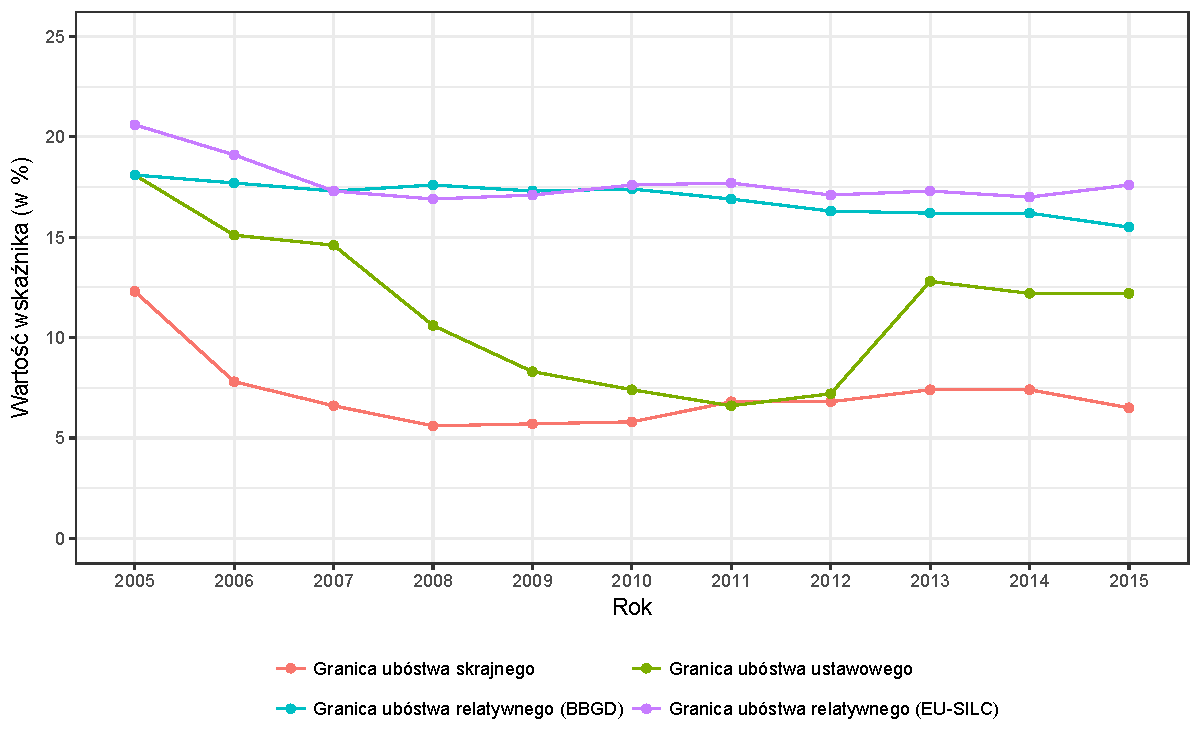
\includegraphics[width=\textwidth]{01_wykresy/gr_stopa_ub-1.pdf}
\caption{Stopa ubóstwa wyznaczona na podstawie różnych granic ubóstwa w latach 2005--2015 w Polsce}
\small{Źródło: opracowanie własne na podstawie danych GUS, IPiSS oraz MRPiPS.}
\label{fig:gr_stopa_ub}
\end{figure}

Ubóstwo skrajne systematycznie malało od roku 2005 do 2008. Przez trzy lata wskaźnik ten kształtował się na stałym poziomie, po czym nastąpił wzrost do poziomu 7,4\% w 2014 roku. Podobny trend można było obserwować w przypadku granicy ubóstwa ustawowego - od roku 2005 do 2011 następował spadek odsetka osób w gospodarstwach domowych zagrożonych ubóstwem ustawowym. W 2011 roku doszło do sytuacji, w której osób dotkniętych skrajnym ubóstwem było więcej od osób uprawnionych do korzystania ze świadczeń pomocy społecznej. W kolejnych latach obserwowany jest wzrost stopy ubóstwa do poziomu 12,2\% w roku 2014. Z kolei zasięg ubóstwa relatywnego jest szacowany w Polsce w oparciu o dwa źródła: Badanie Budżetów Gospodarstw Domowych (BBGD) oraz Europejskie Badanie Dochodów i Warunków Życia (EU-SILC). W pierwszym z nich jako granicę ubóstwa przyjmuje się 50\% średnich wydatków gospodarstw domowych, natomiast w drugim 60\% mediany dochodów. W obu badaniach stosowana jest zmodyfikowana skala ekwiwalentności OECD. Mimo istotnych różnic w zastosowanej metodologii otrzymane wartości zasięgu ubóstwa są do siebie bardzo zbliżone w kolejnych latach. Trend w latach 2005--2015 jest malejący, a największą różnicę odnotowano w roku 2005 (2,5 p.p.). Z kolei w 2007 roku oba oszacowania były identyczne.

Na rysunku \ref{fig:stopa_gleb} zestawiono wartości wskaźników ubóstwa w latach 2005-2015 obliczonych na podstawie badania EU-SILC.

\begin{figure}[ht]
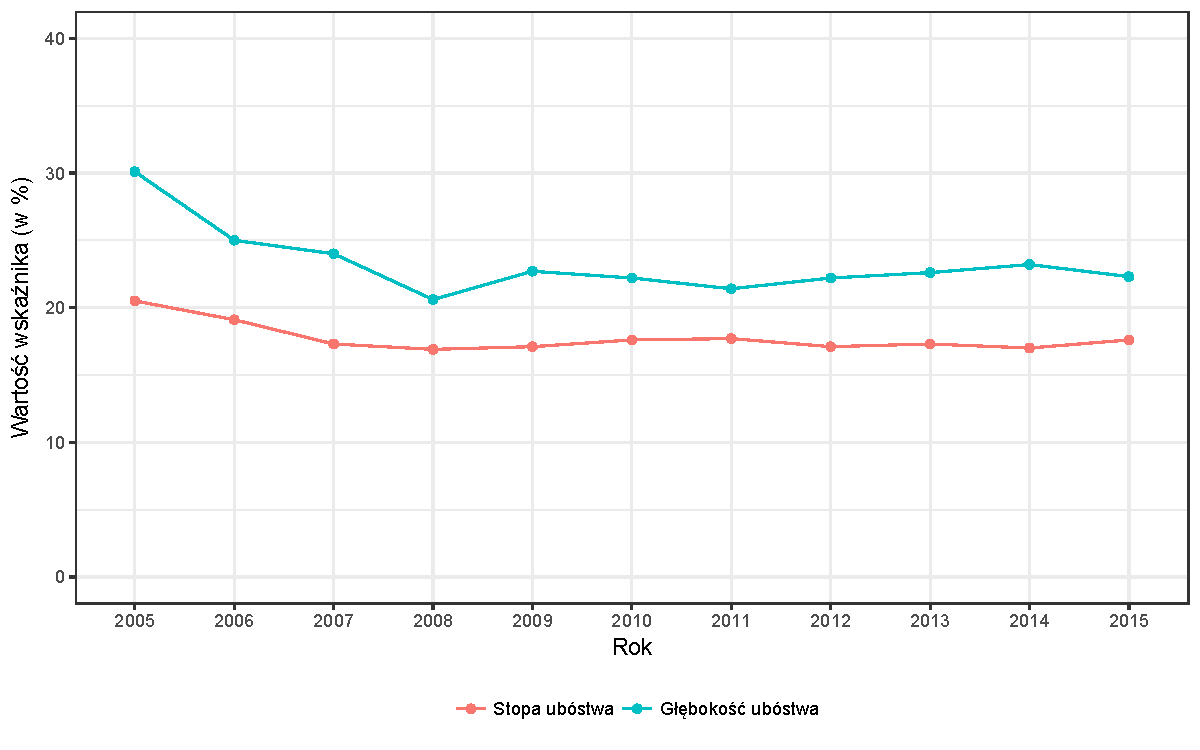
\includegraphics[width=\textwidth]{01_wykresy/stopa_gleb-1.pdf}
\caption{Stopa oraz głębokość ubóstwa w latach 2005--2015 w Polsce}
\small{Źródło: opracowanie własne na podstawie danych Eurostatu.}
\label{fig:stopa_gleb}
\end{figure}

W latach 2005-2015 wartości stopy ubóstwa charakteryzowały się tendencją malejącą - z 20,5\% do 17,0\%. Oznacza to, że w 2015 roku poniżej granicy ubóstwa żyło w Polsce około 6,5 mln osób. Wskaźnik głębokości ubóstwa cechował się występowaniem większych fluktuacji od pozostałych mierników. Wartości luki dochodowej od roku 2005 do roku 2008 systematycznie malały, po czym w 2009 nastąpił wzrost do poziomu 22,7\%. Następnie ponownie wartości głębokości ubóstwa miały tendencję spadkową, aż do roku 2011, kiedy trend ponownie zmienił kierunek. W roku 2014 luka dochowa wynosiła 22,3\%, co oznacza, że dochody osób ubogich były przeciętnie niższe od granicy ubóstwa o 22,3\%. Rosnąca w czasie różnica pomiędzy stopą i głębokością ubóstwa może doprowadzić do tego, że pomimo stałego odsetka osób ubogich, będą one miały coraz niższe dochody.

\subsection{Przestrzenne zróżnicowanie ubóstwa}

Zgodnie z Klasyfikacją Jednostek Terytorialnych do Celów Statystycznych --- NUTS, w Polsce wyróżnia się pięć poziomów terytorialnych. Poziom regionalny obejmuje trzy z nich: makroregiony (NUTS 1), województwa (NUTS 2) i podregiony (NUTS 3). Natomiast na poziomie lokalnym są powiaty (NUTS 4) oraz gminy (NUTS 5). Zgodnie z nomenklaturą UE jednostki lokalne określane są również jako LAU 1 oraz LAU 2 \citep{eurostat2011}. Według stanu na 1 stycznia 2015 r. w~Polsce było 6 jednostek NUTS 1, 16 jednostek NUTS 2, 72 jednostki NUTS 3, 380 jednostek NUTS 4~oraz 3737 jednostek NUTS 5. Wśród ważniejszych modyfikacji klasyfikacji NUTS należy wymienić zmianę z 1 stycznia 2013 r. polegającą na dodaniu jednej jednostki na poziomie NUTS 4 --- miasta na prawach powiatu Wałbrzych oraz zwiększenie liczby podregionów z 66 do 72 w~dniu 1~stycznia 2015 roku.

Dane dotyczące stopy ubóstwa w Polsce publikowane są przez GUS na podstawie BBGD i~EU-SILC. W przypadku pierwszego badania, informacje dostępne są na poziomie całego kraju oraz województw (NUTS 2). Z kolei na podstawie badania EU-SILC w latach 2005--2011 stopa ubóstwa była publikowana na poziomie całego kraju, makroregionów (NUTS 1) oraz województw (NUTS 2), natomiast od roku 2012 zredukowano dostępność szacunków do poziomu kraju oraz makroregionów (NUTS 2).

Na rysunku \ref{fig:arpr_nts2_bbgd_silc_2011} przedstawiono zasięg ubóstwa relatywnego w 2011 roku w województwach Polski według dwóch badań --- BBGD i EU-SILC.

\begin{figure}[ht]
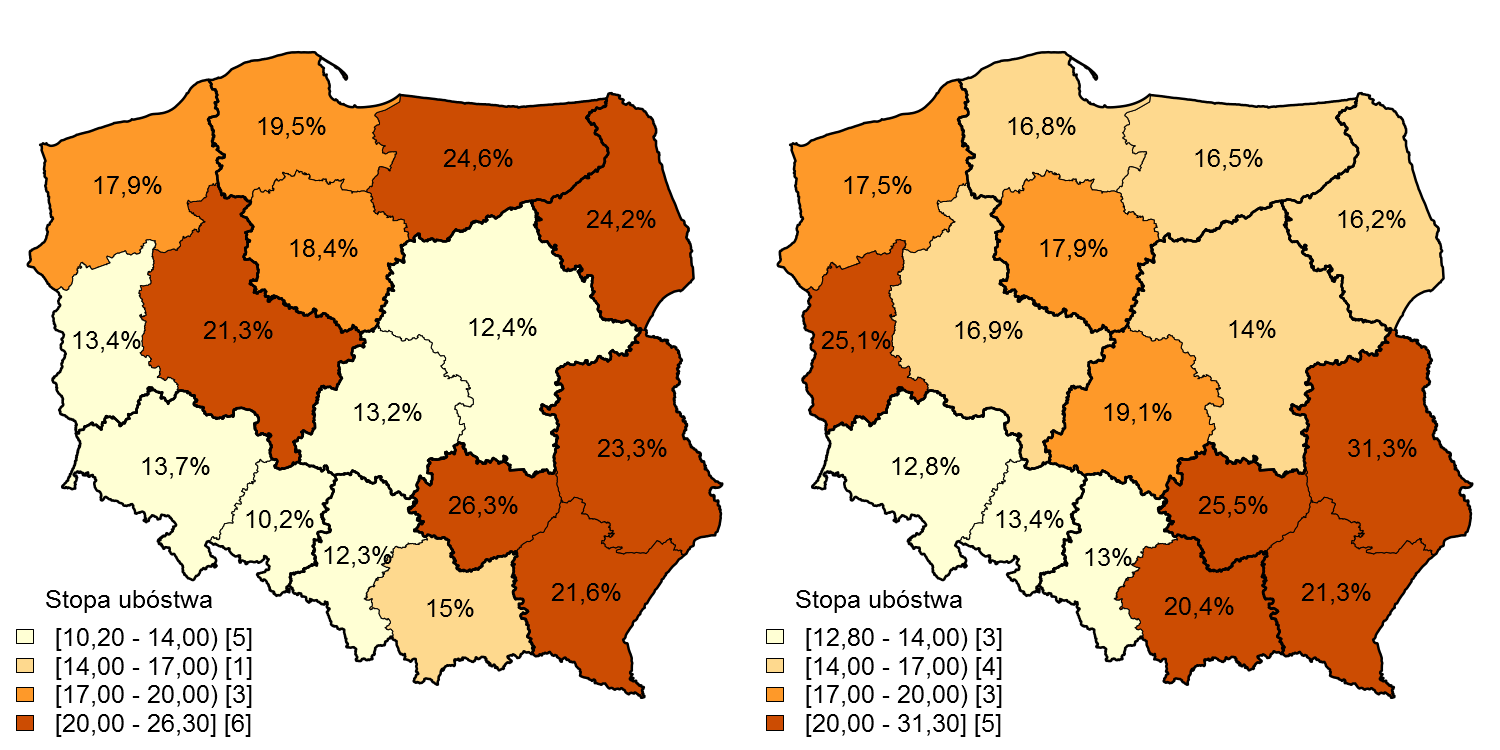
\includegraphics[width=\textwidth]{01_wykresy/arpr_nts2_bbgd_silc_2011.png}
\caption{Stopa ubóstwa na podstawie badania BBGD (po lewej stronie) oraz na podstawie badania EU-SILC (po prawej stronie) w roku 2011 w przekroju województw}
\small{Źródło: opracowanie własne na podstawie BBGD 2011 i EU-SILC 2011.}
\label{fig:arpr_nts2_bbgd_silc_2011}
\end{figure}

Dane zawarte na rysunku \ref{fig:gr_stopa_ub} wskazywały, że pomimo zastosowania różnych kryteriów ubóstwa, wartości stopy ubóstwa nie różniły się znacząco pomiędzy badaniami BBGD oraz EU-SILC. Niemniej analiza tego wskaźnika w przekroju województw uwydatnia istniejące różnice. Największe różnice występują w województwach: lubuskim, łódzkim, małopolskim, podlaskim, warmińsko-mazurskim oraz wielkopolskim. Wspólny dla obu badań jest obraz niskiego ubóstwa na terenach Śląska oraz złej sytuacji gospodarstw w południowo-wschodniej części Polski. Podobne wartości, przeciętnego poziomu ubóstwa, można z kolei zaobserwować w północno-zachodniej części kraju.

Informacje o głębokości ubóstwa nie są publikowane w ujęciu przestrzennym.

\section{Podsumowanie}

W rozdziale przedstawiono definicję ubóstwa oraz sposoby pomiaru tego zjawiska. Wskazano powody, dla których analizy niedostatku nie należy ograniczać wyłącznie do jednego wskaźnika --- stopy ubóstwa. Konieczne jest także wyznaczenie głębokości ubóstwa. Na podstawie literatury przedmiotu oraz badań empirycznych scharakteryzowano główne determinanty ubóstwa. Zaprezentowano także działania pokazujące, że problem ubóstwa nie jest bagatelizowany przez instytucje krajowe oraz międzynarodowe. W ostatnich latach zrealizowano wiele projektów badawczych mających na celu wypracowanie nowych metod analizy ubóstwa oraz estymacji wskaźników niedostatku w szczegółowych przekrojach terytorialnych. 

Na podstawie dostępnych danych pochodzących z badań reprezentacyjnych GUS oraz obliczeń Instytutu Pracy i Spraw Socjalnych, przeanalizowano stosowane w Polsce kryteria ubóstwa w ujęciu czasowym. Biorąc pod uwagę lata 2005--2015 zestawiono ze sobą granice ubóstwa wyznaczane według różnych metod, a następnie na tej podstawie obliczono zasięg ubóstwa. Wykazano wysoką korelację pomiędzy wartościami stopy ubóstwa szacowanej na podstawie dwóch badań reprezentacyjnych --- Badania Budżetów Gospodarstw Domowych oraz Europejskiego Badania Dochodów i Warunków Życia.

Przegląd dostępnych danych w ujęciu przestrzennym pozwolił na identyfikację obszarów mniej i bardziej zagrożonych ubóstwem. Była to jednak analiza na bardzo wysokim stopniu ogólności --- województw, ponieważ na tym poziomie były publikowane wartości stopy ubóstwa. Na tej podstawie nie można było przeprowadzić kompleksowej analizy ubóstwa, ponieważ w tym celu należałoby znać przestrzenny rozkład także głębokości ubóstwa. Ten wskaźnik nie jest publikowany w żadnych przekrojach terytorialnych. 